\documentclass[a4paper]{article}
\usepackage{amsmath,amssymb,algorithmic,booktabs,bm,caption,cases,csvsimple,enumerate,float,geometry,graphicx,indentfirst,makecell,multirow,setspace,tabularx,titlesec}
\captionsetup[figure]{labelsep=period}
\captionsetup[table]{labelsep=period}
\geometry{left=3.5cm,right=3.5cm,top=3.3cm,bottom=3.3cm}
\renewcommand\thesection{\arabic{section}}
\setlength{\parindent}{2em}
\begin{document}
\begin{center}
\huge
\textbf{VE216\\Introduction to Signals and Systems\\}
\Large
\vspace{30pt}
\uppercase{Homework 2}\\
\vspace{5pt}\today\\
\vspace{5pt}
Yihua Liu 518021910998
\vspace{5pt}
\rule[-10pt]{.97\linewidth}{0.05em}
\end{center}

1. Since $f(t)$ is the gain of the system, $y\mathrm{d}t=\mathcal{T}x(t-t_0)=f(t)x(t-t_0)$ while $y(t-t_0)=f(t-t_0)x(t-t_0)$. Since there exists $t_0$, $t_1$ that $f(t_0)\neq f(t_1)$, there exists input signal $x(t)$ and time shift $t_0$ that $y\mathrm{d}t\neq y(t-t_0)$, thus the system is time-invariant, i.e. a system with time-variant gain connot be time-invariant. We can find a counterexample that if $f(t)=t$, $x(t)=\delta(t)$, then $y\mathrm{d}t=t\cdot\delta(t-t_0)\neq(t-t_0)\delta(t-t_0)=y(t-t_0)$, so $x(t)\stackrel{\mathcal{T}}{\longrightarrow}y(t)$ is not a time-invariant system.

2.

(a)
\begin{align*}
    y\mathrm{d}t&=\mathcal{T}x(t-t_0)\\
    &=\int_{-\infty}^t\bigg[\int_{-\infty}^sx(\tau-t_0-5)\mathrm{d}\tau\bigg]\mathrm{d}s\\
    &=\int_{-\infty}^t\bigg[\int_{-\infty}^{s-t_0}x(\tau'-5)\mathrm{d}\tau'\bigg]\mathrm{d}s\\
    &=\int_{-\infty}^{t-t_0}\bigg[\int_{-\infty}^{s'}x(\tau'-5)\mathrm{d}\tau'\bigg]\mathrm{d}s'
\end{align*}
$$y(t-t_0)=\int_{-\infty}^{t-t_0}\bigg[\int_{-\infty}^{s}x(\tau-5)\mathrm{d}\tau\bigg]\mathrm{d}s$$
Since $y\mathrm{d}t=y(t-t_0)$, this system is time-invariant. Since $y(t)$ is linear, $y(t)$ is an LTI system, the impulse response of this system is the output when the input is an impulse signal, i.e.,
$$\boxed{h(t)=\int_{-\infty}^t\bigg[\int_{-\infty}^s\delta(\tau-5)\mathrm{d}\tau\bigg]\mathrm{d}s=\int_{-\infty}^tu(s-5)\mathrm{d}s=(t-5)u(t-5).}$$

(b)
$$y\mathrm{d}t=\int_{-1}^3e^{-(t-\tau)^2}x(\tau-t_0)\mathrm{\tau}=\int_{-1-t_0}^{3-t_0}e^{-(t-t_0-\tau')^2}x(\tau')\mathrm{d}\tau'$$
$$y(t-t_0)=\int_{-1}^3e^{-(t-t_0-\tau)^2}x(\tau)\mathrm{d}\tau$$
Since there exists $x(t)$, $t_0$ that $y\mathrm{d}t\neq y(t-t_0)$, $\boxed{\text{this system is NOT time-invariant}}$.

(c)
\begin{align*}
    y\mathrm{d}t&=\int_{-3}^3\tau^2x(t-t_0-\tau)\mathrm{d}\tau+\int_{-\infty}^{t+1}(t-\tau+3)^{-2}x(\tau-t_0)\mathrm{d}\tau\\
    &=\int_{-3}^3\tau^2x(t-t_0-\tau)\mathrm{d}\tau+\int_{-\infty}^{t-t_0+1}(t-t_0-\tau'+3)^{-2}x(\tau')\mathrm{d}\tau'
\end{align*}
$$y(t-t_0)=\int_{-3}^3\tau^2x(t-t_0-\tau)\mathrm{d}\tau+\int_{-\infty}^{t-t_0+1}(t-t_0-\tau+3)^{-2}x(\tau)\mathrm{d}\tau$$
Since $y\mathrm{d}t=y(t-t_0)$, this system is time-invariant. Since $y(t)$ is linear, $y(t)$ is an LTI system, the impulse response of this system is
\begin{align*}
    h(t)&=\int_{-3}^3\tau^2\delta(t-\tau)\mathrm{d}\tau+\int_{-\infty}^{t+1}(t-\tau+3)^{-2}\delta(\tau)\mathrm{d}\tau\\
    &=\int_{-3}^3t^2\delta(\tau)\mathrm{d}\tau+\int_{-\infty}^{t+1}(t+3)^{-2}\delta(\tau)\mathrm{d}\tau\\
    &=t^2\cdot\mathrm{rect}(\frac{t}{6})+(t+3)^{-2}u(t+1)\\
    &=\left\{
        \begin{array}{lcl}
            0&&{t<-3}\\
            t^2&&{-3\leq t<-1}\\
            t^2+(t+3)^{-2}&&{-1\leq t\leq3}\\
            (t+3)^{-2}&&{t>3}
        \end{array}
    \right.
\end{align*}

3.

(a) If $y(t)=h(t)*x(t)$, i.e.
$$y(t)=\int_{-\infty}^{+\infty} x(\tau)h(t-\tau)\mathrm{d}\tau,$$
then by commutative property and associative property
$$h(t)*x(t-3)=[x(t)*\delta(t-3)]*h(t)=[x(t)*h(t)]*\delta(t-3)=y(t)*\delta(t-3)=y(t-3),$$
Hence, if $y(t)=h(t)*x(t)$ then $\boxed{y(t-3)=h(t)*x(t-3)}$.

(b) For example, if $x(t)=e^{-at}u(t)$ and $h(t)=u(t)$, then when $t>0$
$$x(\tau)h(t-\tau)=\left\{
    \begin{array}{lcl}
        e^{-a\tau},&&0<\tau<t\\
        0,&&\text{other}
    \end{array}
\right.$$
and when $t<0$, $y(t)=0$. When $t>0$,
$$y(t)=\int_0^te^{-a\tau}\mathrm{d}\tau=-\frac{1}{a}e^{-a\tau}\bigg|_0^t=\frac{1}{a}(1-e^{-at}),$$
so for all of $t$,
$$y(t)=\frac{1}{a}(1-e^{-at})u(t),$$
$$y(t-3)=\frac{1}{a}(1-e^{-a(t-3)})u(t-3).$$
Next, we can see $x(t-3)=e^{-a(t-3)}u(t-3)$, $h(t-3)=u(t-3)$, then when $t>6$
$$x(\tau-3)h(t-\tau-3)=\left\{
    \begin{array}{lcl}
        e^{-a(\tau-3)},&&3<\tau<t-3\\
        0,&&\text{other}
    \end{array}
\right.$$
and when $t<6$, $y(t)=0$. When $t>6$,
$$h(t-3)*x(t-3)=\int_3^{t-3}e^{-a(\tau-3)}\mathrm{d}\tau=-\frac{1}{a}e^{-a(\tau-3)}\bigg|_3^{t-3}=\frac{1}{a}(1-e^{-a(t-6)}),$$
so for all of $t$,
$$h(t-3)*x(t-3)=\frac{1}{a}(1-e^{-a(t-6)})u(t-6).$$
Therefore, $\boxed{y(t-3)\neq h(t-3)*x(t-3)}$.

(c) To repeat (a) and (b) for multiplication, we first give a simple proof of the correct statement. If $y(t)=h(t)\cdot x(t)$, then by time-shifting we can directly derive that
$$y(t-3)=h(t-3)\cdot x(t-3).$$
To give a counterexample for the incorrect statement, we assume that $x(t)=u(t)$, $h(t)=\delta(t)$, then $y(t)=h(t)\cdot x(t)=\delta(t)$, $y(t-3)=\delta(t-3)$,
$$h(t)\cdot x(t-3)=\delta(t)\cdot u(t-3)=0\neq y(t-3).$$
Therefore, $y(t)=h(t)\cdot x(t)$ does not imply that $y(t-3)=h(t)\cdot x(t-3)$.

4.

(a) By the definition of convolution integral, the range that $y(t)$ is non-zero must at least start at $a+c$. After conversion, $x_2(t-\tau)$ is non-zero over the range $t-d\leq t\leq t-c$. Considering the product of $x_1(\tau)$ and $x_2(t-\tau)$, when shifting $x_2(t-\tau)$ from $t-c=-\infty$ to $a$, $x_1(\tau)x_2(t-\tau)$ is zero. Then, the product will become non-zero until $x_2(t-\tau)$ is shifted to $t-d>b$, so the range ends at $t=b+d$. Therefore, the range of values of $t$ for which $y(t)$ is possibly non-zero is $\boxed{a+c\leq t\leq b+d}$.

(b) Using $\text{rect}(t)=u(t+1/2)-u(t-1/2)$, we have
$$\text{rect}((t-2)/2)=u(t-1)-u(t-3)$$
$$\text{rect}((t+3)/4)=u(t+5)-u(t+1)$$
so
\[\arraycolsep=1.4pt\def\arraystretch{1.2}
\begin{array}{ll}
    &\text{rect}((t-2)/2)*\text{rect}((t+3)/4)\\
    =&[u(t-1)-u(t-3)]*[u(t+5)-u(t+1)]\\
    =&u(t-1)*u(t+5)-u(t-1)*u(t+1)-u(t-3)*u(t+5)+u(t-3)*u(t+1)\\
    &\qquad\text{(Distributive property)}
\end{array}
\]
The convolution integral of unit step function and unit step function is unit ramp function denoted as $R(t)$
$$u(t)*u(t)=\int_{-\infty}^{+\infty}u(\tau)u(t-\tau)=tu(t)=R(t)$$
We can prove the time-shifting property of convolution integral
\begin{align*}
    h(t-t_1)*x(t-t_2)&=[x(t)*\delta(t-t_2)]*[h(t)*\delta(t-t_1)]\\
    &=[x(t)*h(t)]*[\delta(t-t_1)*\delta(t-t_2)]\\
    &=y(t)*\delta(t-t_1-t_2)\\
    &=y(t-t_1-t_2)
\end{align*}
Thus,
$$u(t-t_1)*u(t-t_2)=R(t-t_1-t_2).$$
Thus,
\[\arraycolsep=1.4pt\def\arraystretch{1.2}
\begin{array}{ll}
    &\text{rect}((t-2)/2)*\text{rect}((t+3)/4)\\
    =&R(t+4)-R(t)-R(t+2)+R(t-2)\\
    =&(t+4)u(t+4)-tu(t)-(t+2)u(t+2)+(t-2)u(t-2)\\
    =&%\left\{\arraycolsep=6pt\def\arraystretch{1}
        \begin{cases}
            0&{t<-4}\\
            t+4&{-4\leq t<-2}\\
            2&{-2\leq t<0}\\
            -t+2&{0\leq t<2}\\
            0&{t\geq2}
        \end{cases}
    %\right.
\end{array}
\]
\begin{figure}[H]
    \begin{center}
        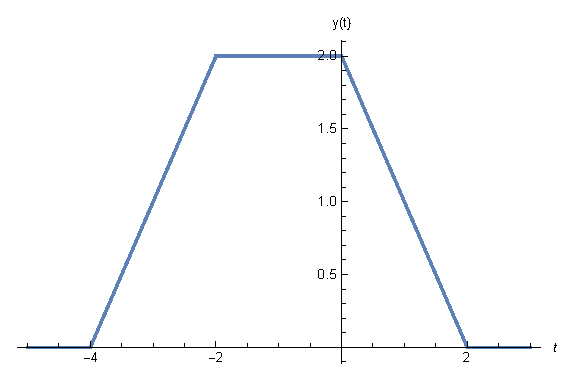
\includegraphics[width=0.6\textwidth]{4(b).eps}
    \end{center}
    \caption{Sketch of $\text{rect}((t-2)/2)*\text{rect}((t+3)/4)$.}
\end{figure}
We can see that the non-zero range of the convolution integral is $-4<t<2$. $\text{rect}((t-2)/2)$ is non-zero over the range $1<t<3$ and $\text{rect}((t+3)/4)$ is non-zero over the range $-5<t<-1$, so $a=1$, $b=3$, $c=-5$, $d=-1$, $a+c=-4$, $b+d=2$, according to (a) the non-zero range is $-4<t<2$, which is exactly what we have, so our result in part (a) is true.

5.

(a) The response $y(t)$ is
$$y(t)=\int_{-\infty}^\infty x(\tau)\mathrm{d}\tau=\int_{-\infty}^\infty e^{-\alpha\tau}u(\tau)e^{-\beta(t-\tau)}u(t-\tau)\mathrm{d}\tau.$$
Since
\[u(\tau)=
    \begin{cases}
        1,&t-\tau\geq0\\
        0,&\text{otherwise}
    \end{cases}
\]
and
\[u(t-\tau)=
    \begin{cases}
        1,&\tau\leq t\\
        0,&\text{otherwise}
    \end{cases}
\]
we can change the limit of the integral and simply the expression:
\begin{align*}
    y(t)&=\int_{-\infty}^\infty e^{-\alpha\tau}u(\tau)e^{-\beta(t-\tau)}u(t-\tau)\mathrm{d}\tau\\
    &=\int_0^\infty e^{-\alpha\tau}e^{-\beta(t-\tau)}u(t-\tau)\mathrm{d}\tau\\
    &=\int_0^t e^{-\alpha\tau-\beta(t-\tau)}\mathrm{d}\tau\\
    &=\int_0^t e^{-(\alpha-\beta)\tau}e^{-\beta t}\mathrm{d}\tau\\
\end{align*}
When $\alpha\neq\beta$, we calculate the integral as
\begin{align*}
    y(t)&=e^{-\beta t}\int_0^te^{-(\alpha-\beta)\tau}\mathrm{d}\tau\\
    &=e^{-\beta t}\frac{e^{-(\alpha-\beta)\tau}}{-(\alpha-\beta)}\bigg|_0^t\\
    &=\frac{e^{-\beta t}}{\beta-\alpha}(e^{(\beta-\alpha)t}-1)\\
    &=\frac{e^{-\alpha t}-e^{-\beta t}}{\beta-\alpha}
\end{align*}
When $\alpha=\beta$,
\begin{align*}
    y(t)&=\int_0^t e^{-(\alpha-\alpha)\tau}e^{-\alpha t}\mathrm{d}\tau\\
    &=\int_0^t e^{-\alpha t}\mathrm{d}\tau\\
    &=te^{-\alpha t}
\end{align*}
Since the convolution exists from 0 to $\infty$, the response $y(t)$ is
\[\boxed{y(t)=
    \begin{cases}
        \dfrac{e^{-\alpha t}-e^{-\beta t}}{\beta-\alpha}u(t),&\alpha\neq\beta\\
        te^{-\alpha t}u(t),&\alpha=\beta
    \end{cases}}
\]
\begin{figure}[H]
    \begin{center}
        \includegraphics[width=0.6\textwidth]{5(a)-1.eps}
    \end{center}
    \caption{Sketch of $y(t)$ when $\alpha=1$ and $\beta=2$.}
\end{figure}
\begin{figure}[H]
    \begin{center}
        \includegraphics[width=0.6\textwidth]{5(a)-2.eps}
    \end{center}
    \caption{Sketch of $y(t)$ when $\alpha=\beta=1$.}
\end{figure}

(b) According to the provided conditions, $x(t)=at+b$ and $h(t)=\frac{4}{3}(u(t)-u(t-1))-\frac{1}{3}\delta(t-2)$, then
$$x(\tau)=a\tau+b$$
$$h(t-\tau)=\frac{4}{3}(u(t-\tau)-u(t-\tau-1))-\frac{1}{3}\delta(t-\tau-2)$$
The response
\begin{align*}
    y(t)&=x(t)*h(t)\\
    &=x(t)*(\frac{4}{3}(u(t)-u(t-1))-\frac{1}{3}\delta(t-2))\\
    &=\frac{4}{3}x(t)*(u(t)-u(t-1))-\frac{1}{3}x(t)*\delta(t-2)\\
    &=\frac{4}{3}\int_{-\infty}^\infty(a\tau+b)(u(t-\tau)-u(t-\tau-1))\mathrm{d}\tau-\frac{1}{3}\int_{-\infty}^\infty(a\tau+b)\delta(t-\tau-2)\mathrm{d}\tau\\
    &=\frac{4}{3}\int_{t-1}^t(a\tau+b)\mathrm{d}\tau-\frac{1}{3}(a(t-2)+b)\\
    &=\frac{4}{3}(a\frac{\tau^2}{2}+b\tau)\bigg|_{t-1}^t-\frac{1}{3}(a(t-2)+b)\\
    &=\frac{4}{3}(\frac{a}{2}(2t-1)+b)-\frac{1}{3}(at-2a+b)\\
    &=\frac{4}{3}at-\frac{2a}{3}+\frac{4b}{3}-\frac{1}{3}at+\frac{2a}{3}-\frac{b}{3}\\
    &=at+b
\end{align*}
Therefore, the response is $\boxed{y(t)=at+b}$.
\begin{figure}[H]
    \begin{center}
        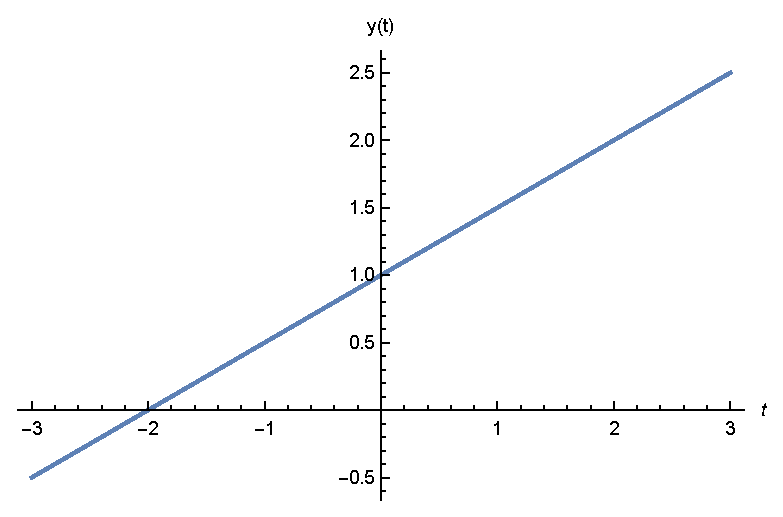
\includegraphics[width=0.6\textwidth]{5(b).eps}
    \end{center}
    \caption{Sketch of $y(t)$ when $a=\frac{1}{2}$ and $b=1$.}
\end{figure}

6.

(a)
$$y\mathrm{d}t=\sum_{n=-\infty}^\infty x(t-t_0)\delta(t-nT)=\sum_{n=-\infty}^\infty x(nT-t_0)$$
$$y(t-t_0)=\sum_{n=-\infty}^\infty x(t-t_0)\delta(t-t_0-nT)=\sum_{n=-\infty}^\infty x(nT)$$
Since there exists $x(t)$ and $t_0$ that $y\mathrm{d}t\neq y(t-t_0)$, this system is NOT time-invariant.

(b) To sketch $y(t)$ we would like to deal with $x(t)$ first.
\begin{align*}
    y(t)&=\sum_{k=-\infty}^\infty\delta(t-nT)*h(t)\\
    &=\int_{-\infty}^\infty(\sum_{k=-\infty}^\infty\delta(t-nT-\tau))h(\tau)\mathrm{d}\tau\\
    &=\sum_{k=-\infty}^\infty\bigg[\int_{-\infty}^\infty\delta(t-nT-\tau)h(\tau)\mathrm{d}\tau\bigg]\\
    &=\sum_{k=-\infty}^\infty\bigg[\int_{-\infty}^\infty\delta(nT+\tau-t)h(\tau)\mathrm{d}\tau\bigg]\\
    &=\sum_{k=-\infty}^\infty h(t-nT)
\end{align*}
Here we use the time shift property of impulse signal
$$\int_{-\infty}^\infty x(\tau)\delta(t-\tau)\mathrm{d}\tau=\int_{-\infty}^\infty x(t)\delta(t-\tau)\mathrm{d}\tau=x(t)\int_{-\infty}^\infty\delta(t-\tau)\mathrm{d}\tau=x(t).$$
Then, we would like to sketch $y(t)$ for different values of $T$ respectively.
\begin{figure}[H]
    \begin{center}
        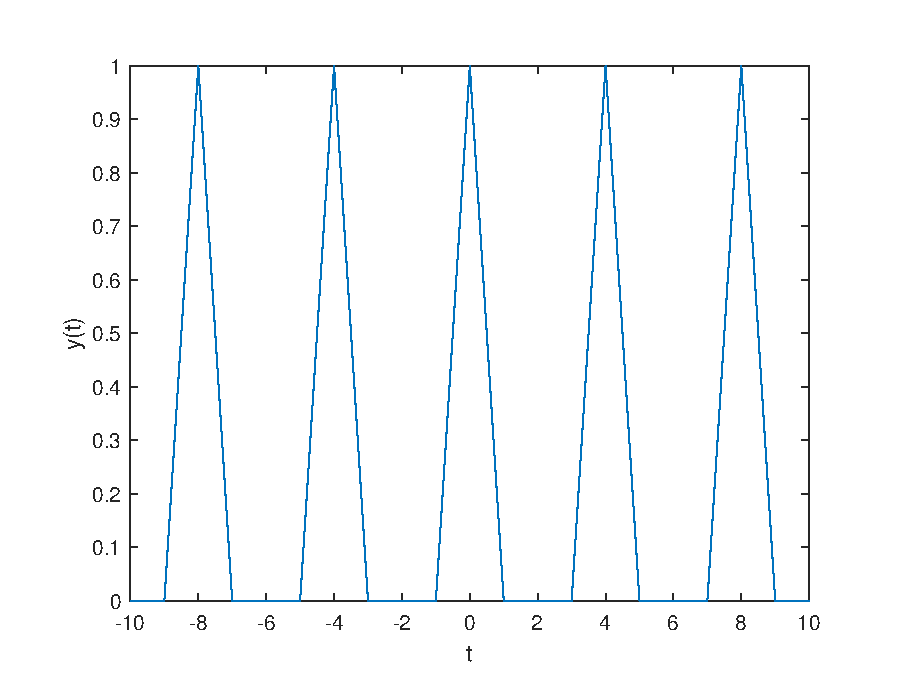
\includegraphics[width=0.8\textwidth]{6(b)-1.eps}
    \end{center}
    \caption{Sketch of $y(t)=\sum_{k=-\infty}^\infty h(t-4T)$ for $T=4$.}
\end{figure}
\begin{figure}[H]
    \begin{center}
        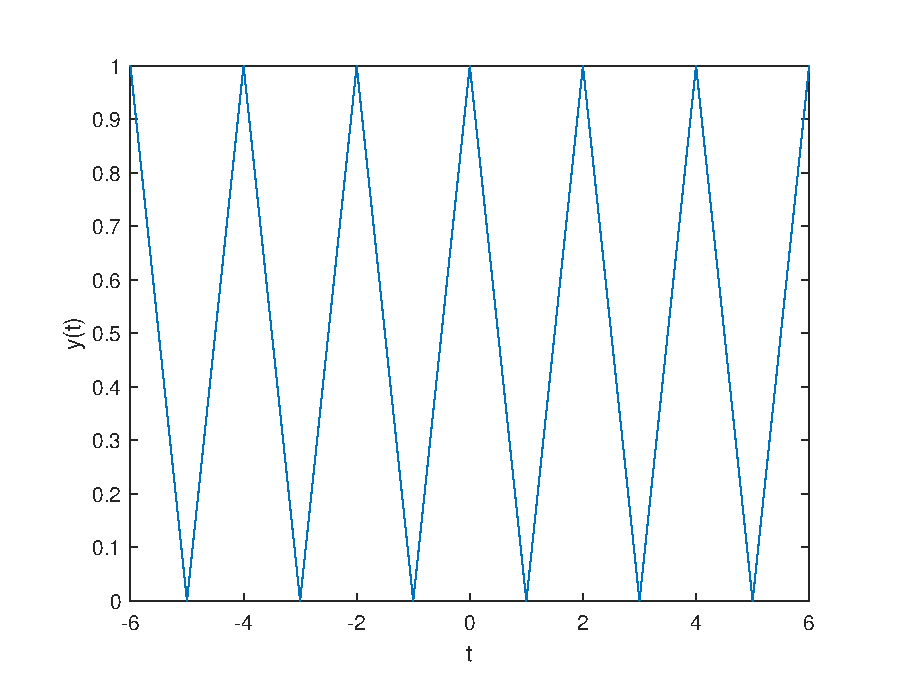
\includegraphics[width=0.8\textwidth]{6(b)-2.eps}
    \end{center}
    \caption{Sketch of $y(t)=\sum_{k=-\infty}^\infty h(t-2T)$ for $T=2$.}
\end{figure}
\begin{figure}[H]
    \begin{center}
        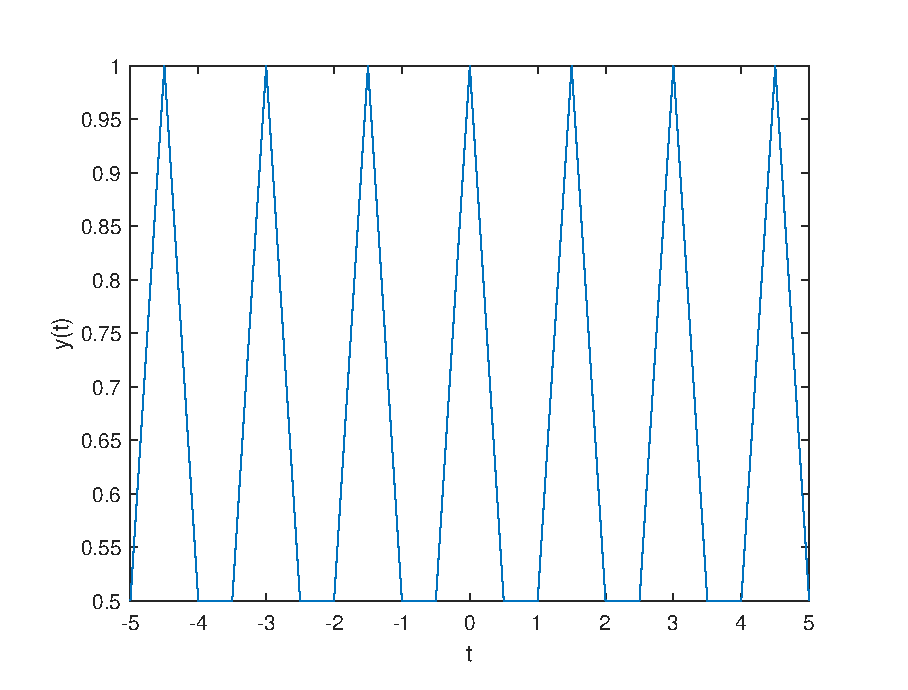
\includegraphics[width=0.8\textwidth]{6(b)-3.eps}
    \end{center}
    \caption{Sketch of $y(t)=\sum_{k=-\infty}^\infty h(t-1.5T)$ for $T=1.5$.}
\end{figure}
\begin{figure}[H]
    \begin{center}
        \includegraphics[width=0.8\textwidth]{6(b)-4.eps}
    \end{center}
    \caption{Sketch of $y(t)=\sum_{k=-\infty}^\infty h(t-T)$ for $T=1$.}
\end{figure}
\newpage
7.
\begin{equation}
    y(t)=(x*h)(t)\Leftrightarrow y(t)=\int_{-\infty}^\infty x(\tau)h(t-\tau)\mathrm{d}\tau
\end{equation}

(a)
By the definition of convolution integral and Fubini's theorem,
\begin{align*}
    \int_{-\infty}^\infty y(t)\mathrm{d}t&=\int_{-\infty}^\infty(x*h)(t)\mathrm{d}t\\
    &=\int_{-\infty}^\infty\bigg[\int_{-\infty}^\infty x(\tau)h(t-\tau)\mathrm{d}\tau\bigg]\mathrm{d}t\\
    &=\int_{-\infty}^\infty x(\tau)\bigg[\int_{-\infty}^\infty h(t-\tau)\mathrm{d}t\bigg]\mathrm{d}\tau
\end{align*}
Substitute $x(t)$ for $x(\tau)$ and $h(t)$ for $h(t-\tau)$ using $\mathrm{d}t=\mathrm{d}(t-\tau)$,
\begin{align*}
    \int_{-\infty}^\infty y(t)\mathrm{d}t&=\int_{-\infty}^\infty x(t)\bigg[\int_{-\infty}^\infty h(t)\mathrm{d}t\bigg]\mathrm{d}t\\
    &=\bigg[\int_{-\infty}^\infty x(t)\mathrm{d}t\bigg]\bigg[\int_{-\infty}^\infty h(t)\mathrm{d}t\bigg]
\end{align*}

(b) Differentiate both sides of Eq. (1) with respect to $t$,
\begin{align*}
    \frac{\mathrm{d}}{\mathrm{d}t}y(t)&=\frac{\mathrm{d}}{\mathrm{d}t}\bigg[\int_{-\infty}^\infty x(t-\tau)h(\tau)\mathrm{d}\tau\bigg]\\
    &=\int_{-\infty}^\infty\frac{\mathrm{d}}{\mathrm{d}t}[x(t-\tau)h(\tau)]\mathrm{d}\tau\\
    &=\int_{-\infty}^\infty h(\tau)\bigg[\frac{\mathrm{d}}{\mathrm{d}t}x(t-\tau)\bigg]\mathrm{d}\tau\\
    &=\bigg[\frac{\mathrm{d}}{\mathrm{d}t}x(t)\bigg]*h(t)
\end{align*}
\begin{align*}
    \frac{\mathrm{d}}{\mathrm{d}t}y(t)&=\frac{\mathrm{d}}{\mathrm{d}t}\bigg[\int_{-\infty}^\infty h(t-\tau)x(\tau)\mathrm{d}\tau\bigg]\\
    &=\int_{-\infty}^\infty\frac{\mathrm{d}}{\mathrm{d}t}[h(t-\tau)x(\tau)]\mathrm{d}\tau\\
    &=\int_{-\infty}^\infty x(\tau)\bigg[\frac{\mathrm{d}}{\mathrm{d}t}h(t-\tau)\bigg]\mathrm{d}\tau\\
    &=x(t)*\bigg[\frac{\mathrm{d}}{\mathrm{d}t}h(t)\bigg]
\end{align*}
Therefore,
\begin{equation}
    \frac{\mathrm{d}}{\mathrm{d}t}y(t)=\bigg[\frac{\mathrm{d}}{\mathrm{d}t}x(t)\bigg]*h(t)=x(t)*\bigg[\frac{\mathrm{d}}{\mathrm{d}t}h(t)\bigg]    
\end{equation}

8.

(a) Using results from Problem 5(a),
\begin{align*}
    u(t)*u(t)&=\int_{-\infty}^\infty u(\tau)u(t-\tau)\mathrm{d}\tau\\
    &=\int_0^t1\cdot1\mathrm{d}\tau\\
    &=t.
\end{align*}
Since the convolution exists from 0 to $\infty$, $u(t)$ is multiplied to the terms
$$\boxed{u(t)*u(t)=tu(t).}$$

(b)
\begin{align*}
    u(t)*t^2u(t)&=\int_{-\infty}^\infty \tau^2u(\tau)u(t-\tau)\mathrm{d}\tau\\
    &=\int_0^tt^2\cdot1\mathrm{d}\tau\\
    &=\frac{1}{3}t^3.
\end{align*}
Since the convolution exists from 0 to $\infty$,
$$\boxed{u(t)*t^2u(t)=\frac{1}{3}t^3u(t).}$$

9. We would like to use the result of Problem 7(b) that $\frac{\mathrm{d}}{\mathrm{d}t}y(t)=[\frac{\mathrm{d}}{\mathrm{d}t}x(t)]*h(t)$. Since $x(t)=u(t)$ and $y(t)=(3-t)\text{rect}(\frac{t-1}{2})=(3-t)(u(t)-u(t-2))$, the derivatives of $x(t)$ and $y(t)$ are respectively
$$\frac{\mathrm{d}}{\mathrm{d}t}x(t)=\delta(t)$$
$$\frac{\mathrm{d}}{\mathrm{d}t}y(t)=(3-t)(\delta(t)-\delta(t-2))-u(t)+u(t-2)$$
Applying Eq. (2),
$$\frac{\mathrm{d}}{\mathrm{d}t}y(t)=\delta(t)*h(t)=\int_{-\infty}^\infty\delta(t-\tau)h(\tau)\mathrm{d}\tau=h(t)$$
Therefore, the impulse response of the system is
$$\boxed{h(t)=(3-t)(\delta(t)-\delta(t-2))-u(t)+u(t-2))}$$

10.

(a) For any signals $x_1(t)$, $x_2(t)$ and any constants $a_1$ and $a_2$,
$$\mathcal{T}[x_1(t)]=x_1(\sin(t))$$
$$\mathcal{T}[x_2(t)]=x_2(\sin(t))$$
$$\alpha\mathcal{T}[x_1(t)]+\beta\mathcal{T}[x_2(t)]=\alpha x_1(\sin(t))+\beta x_2(\sin(t))$$
$$\mathcal{T}[\alpha x_1(t)+\beta x_2(t)]=\alpha x_1(\sin(t))+\beta x_2(\sin(t))$$
$$\mathcal{T}[\alpha x_1(t)+\beta x_2(t)]=\alpha\mathcal{T}[x_1(t)]+\beta\mathcal{T}[x_2(t)]$$
Therefore, the system is $\boxed{\text{linear}}$.

Since $\forall t\ \mathrm{ran}\sin(t)=[-1,1]\subset\mathrm{ran}\ t$, if $\exists M_x$ s.t. $|x(t)|\leq M_x<\infty\ \forall t$, then there must exist an $M_y$ s.t.
$$|y(t)|\leq M_y<\infty\ \forall t.$$
Therefore, the system is $\boxed{\text{stable}}$.

Since the output $y(t)$ at any time $t$ may depend on previous and future values of the input signal, the system is $\boxed{\text{NOT causal}}$ and $\boxed{\text{NOT memoryless}}$.
$$y\mathrm{d}t=x(\sin(t)-t_0)\neq x(\sin(t-t_0))=y(t-t_0)$$
Therefore, the system is $\boxed{\text{NOT time-invariant}}$.

(b) For any signals $x_1(t)$, $x_2(t)$ and any constants $a_1$ and $a_2$,
$$\mathcal{T}[x_1(t)]=\frac{\mathrm{d}}{\mathrm{d}t}(e^{-t}x_1(t))$$
$$\mathcal{T}[x_2(t)]=\frac{\mathrm{d}}{\mathrm{d}t}(e^{-t}x_2(t))$$
$$\alpha\mathcal{T}[x_1(t)]+\beta\mathcal{T}[x_2(t)]=\alpha\frac{\mathrm{d}}{\mathrm{d}t}(e^{-t}x_1(t))+\beta\frac{\mathrm{d}}{\mathrm{d}t}(e^{-t}x_2(t))$$
$$\mathcal{T}[\alpha x_1(t)+\beta x_2(t)]=\frac{\mathrm{d}}{\mathrm{d}t}(e^{-t}(\alpha x_1(t)+\beta x_2(t))=\alpha\frac{\mathrm{d}}{\mathrm{d}t}(e^{-t}x_1(t))+\beta\frac{\mathrm{d}}{\mathrm{d}t}(e^{-t}x_2(t))$$
$$\mathcal{T}[\alpha x_1(t)+\beta x_2(t)]=\alpha\mathcal{T}[x_1(t)]+\beta\mathcal{T}[x_2(t)]$$
Therefore, the system is $\boxed{\text{linear}}$.

If we take a bounded input signal $x(t)=\sin(\frac{1}{t})$ so that $-1\leq x(t)\leq1$, then
$$y(t)=\frac{\mathrm{d}}{\mathrm{d}t}[e^{-t}x(t)]=-e^{-t}(\frac{\cos\frac{1}{t}}{t^2}+\sin\frac{1}{t})$$
Since $\lim_{t\rightarrow-\infty}y(t)=+\infty$, $y(t)$ is unbounded, i.e. there does not exist an $M_y$ s.t. $|y(t)|\leq M_y<\infty\ \forall t$, so the system is $\boxed{\text{NOT stable}}$.

Since we can express $y(t)$ as
$$y(t)=\bigg(\frac{\mathrm{d}x(t)}{\mathrm{d}t}-x(t)\bigg)e^{-t}$$
we see that its causality and memory are the same as those of the system in Homework 1 Problem 10(e), again according to the definition of derivative, the output $y(t)$ at any time $t$ may depend on previous and present values of the input signal, the system is $\boxed{\text{causal}}$ and $\boxed{\text{NOT memoryless}}$.

$$y\mathrm{d}t=\frac{\mathrm{d}}{\mathrm{d}t}[{e^{-t}}x(t-t_0)]\neq\frac{\mathrm{d}}{\mathrm{d}t}[e^{-(t-t_0)}x(t-t_0)]=y(t-t_0)$$
Therefore, the system is $\boxed{\text{NOT time-invariant}}$.

11.

(a) The input signal $x_2(t)$ is
$$x_2(t)=x_1(t)-x_1(t-2),$$
so the response of the system can be determined by
$$y_2(t)=y_1(t)-y_1(t-2)=2(1-|t-1|)(u(t)-u(t-2))-2(1-|t-3|)(u(t-2)-u(t-4)).$$
\begin{figure}[H]
    \begin{center}
        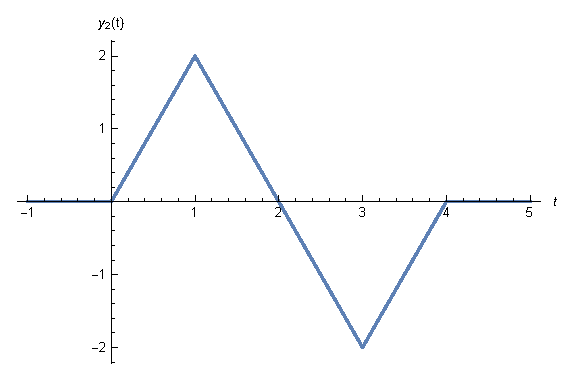
\includegraphics[width=0.6\textwidth]{11(a).eps}
    \end{center}
    \caption{Sketch of the response of the system to the input $x_2(t)$.}
\end{figure}

(b) The input signal $x_3(t)$ is
$$x_3(t)=x_1(t)+x_1(t+1),$$
so the response of the system can be determined by
$$y_3(t)=y_1(t)+y_1(t+1)=2(1-|t-1|)(u(t)-u(t-2))+2(1-|t|)(u(t+1)-u(t-1)).$$
\begin{figure}[H]
    \begin{center}
        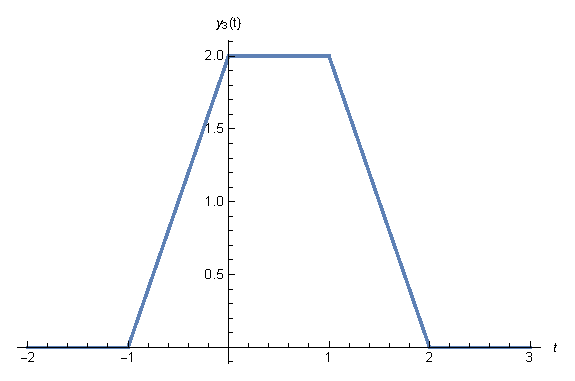
\includegraphics[width=0.6\textwidth]{11(b).eps}
    \end{center}
    \caption{Sketch of the response of the system to the input $x_3(t)$.}
\end{figure}
12. Since the two signals are complex interpreted by the unit step functions, we would like to compute the convolution by graphs. Denote $x_1(t)=\mathrm{tri}(\frac{t}{2})$ and $x_2(t)=\mathrm{rect}(\frac{t-1}{2})$.
\begin{figure}[H]
    \begin{center}
        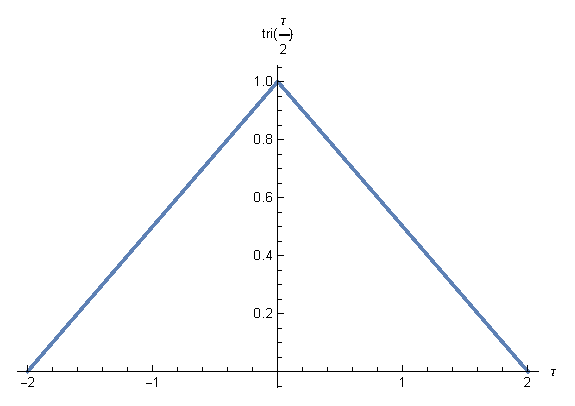
\includegraphics[width=0.6\textwidth]{12-1.eps}
    \end{center}
    \caption{$x_1(\tau)=\mathrm{tri}(\frac{\tau}{2})$.}
\end{figure}
\begin{figure}[H]
    \begin{center}
        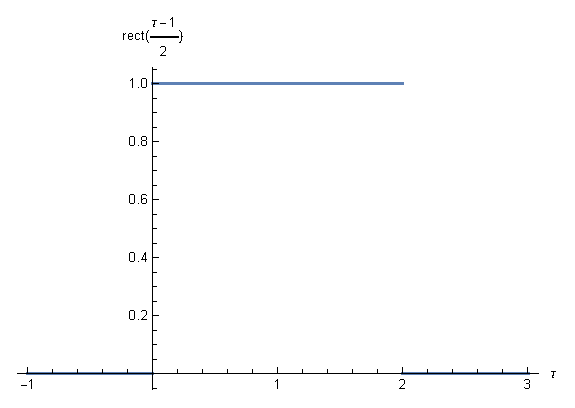
\includegraphics[width=0.55\textwidth]{12-2.eps}
    \end{center}
    \caption{$x_2(\tau)=\mathrm{rect}(\frac{\tau-1}{2})$.}
\end{figure}
\begin{figure}[H]
    \begin{center}
        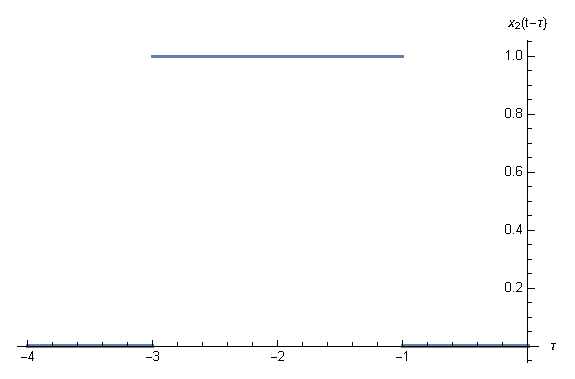
\includegraphics[width=0.55\textwidth]{12-3.eps}
    \end{center}
    \caption{$x_2(t-\tau)$ when $t=-1$.}
\end{figure}

When $t\leq-2$, $x_1(t)*x_2(t)=0$.
\begin{figure}[H]
    \begin{center}
        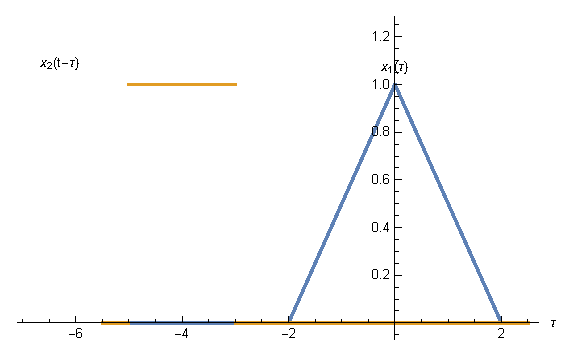
\includegraphics[width=0.8\textwidth]{12-4.eps}
    \end{center}
    \caption{$x_1(\tau)$ and $x_2(t-\tau)$ when $t=-3$.}
\end{figure}
\newpage
When $-2\leq t\leq0$,
\begin{figure}[H]
    \begin{center}
        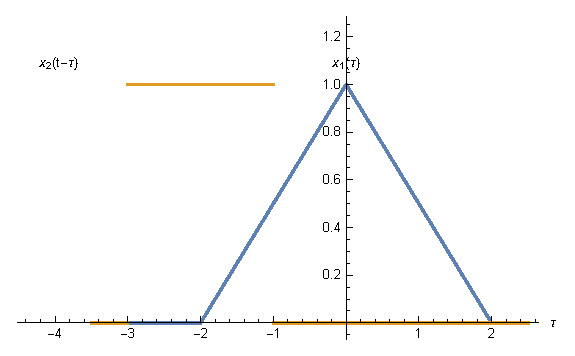
\includegraphics[width=0.8\textwidth]{12-5.eps}
    \end{center}
    \caption{$x_1(\tau)$ and $x_2(t-\tau)$ when $t=-1$.}
\end{figure}
$$x_1(t)*x_2(t)=\int_{-2}^t\bigg(\frac{1}{2}\tau+1\bigg)\cdot1\mathrm{d}\tau=\bigg(\frac{\tau^2}{4}+\tau\bigg)\bigg|_{-2}^t=\frac{1}{4}(t+2)^2.$$

When $0\leq t\leq2$,
\begin{figure}[H]
    \begin{center}
        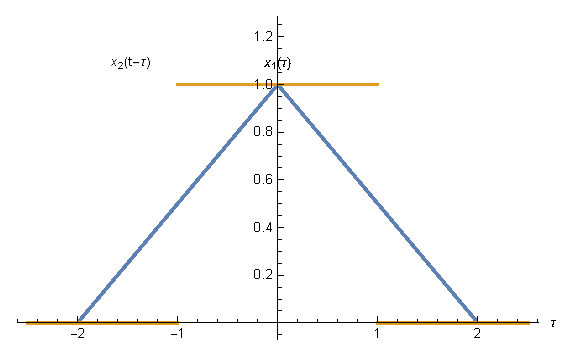
\includegraphics[width=0.8\textwidth]{12-6.eps}
    \end{center}
    \caption{$x_1(\tau)$ and $x_2(t-\tau)$ when $t=1$.}
\end{figure}
$$x_1(t)*x_2(t)=\int_{t-2}^t\bigg(-\frac{1}{2}|\tau|+1\bigg)\cdot1\mathrm{d}\tau=-\bigg(\frac{1}{4}|\tau|^2-|\tau|\bigg)\bigg|_{t-2}^t=-\frac{1}{2}t^2+t+1.$$
\newpage
When $2\leq t\leq4$,
\begin{figure}[H]
    \begin{center}
        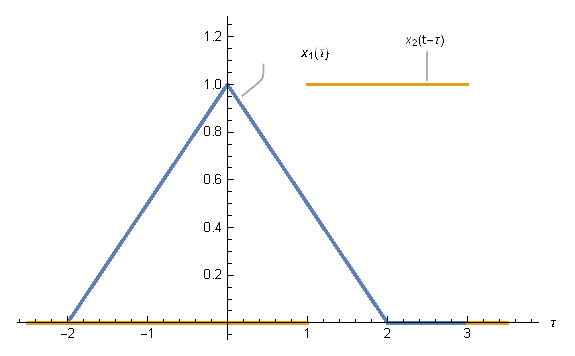
\includegraphics[width=0.8\textwidth]{12-7.eps}
    \end{center}
    \caption{$x_1(\tau)$ and $x_2(t-\tau)$ when $t=3$.}
\end{figure}
%\begin{align*}
%    x_1(t)*x_2(t)&=\frac{1}{2}(t+1)^2u(t+1)-t^2u(t)+\int_2^t(((\tau-2)+1)-(-(\tau-2)+1))\cdot1\mathrm{d}\tau\\
%    &=\frac{1}{2}(t+1)^2u(t+1)-t^2u(t)+(t^2-4t)\bigg|_2^t\\
%    &=\frac{1}{2}(t+1)^2u(t+1)-t^2u(t)+t^2-4t+4\\
%    &=\frac{1}{2}(t+1)^2u(t+1)-t^2u(t)+(t-2)^2u(t-2)
%\end{align*}
$$x_1(t)*x_2(t)=\int_{t-2}^2\bigg(-\frac{1}{2}\tau+1\bigg)\cdot1\mathrm{d}\tau=-\bigg(\frac{1}{4}\tau^2-\tau\bigg)\bigg|_{t-2}^2=\frac{1}{4}(t-4)^2.$$

When $t\geq4$,
\begin{figure}[H]
    \begin{center}
        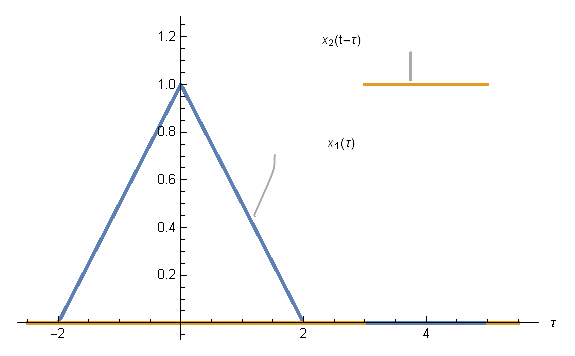
\includegraphics[width=0.7\textwidth]{12-8.eps}
    \end{center}
    \caption{$x_1(\tau)$ and $x_2(t-\tau)$ when $t=5$.}
\end{figure}
%\begin{align*}
%    x_1(t)*x_2(t)&=\frac{1}{2}(t+1)^2u(t+1)-t^2u(t)+(t-2)^2u(t-2)+\int_3^t(-(\tau-2)+1)\cdot1\mathrm{d}\tau\\
%    &=\frac{1}{2}(t+1)^2u(t+1)-t^2u(t)+(t-2)^2u(t-2)-\bigg(\frac{1}{2}t^2-3t\bigg)\bigg|_3^t\\
%    &=\frac{1}{2}(t+1)^2u(t+1)-t^2u(t)+(t-2)^2u(t-2)-\frac{1}{2}(t^2+6t-9)\\
%    &=\frac{1}{2}(t+1)^2u(t+1)-t^2u(t)+(t-2)^2u(t-2)-\frac{1}{2}(t-3)^2u(t-3)
%\end{align*}
$$x_1(t)*x_2(t)=0.$$
In fact, we can rewrite the expression as
$$x(t)=\mathrm{tri}(\frac{\tau}{2})*\mathrm{rect}(\frac{\tau-1}{2})=\frac{1}{4}((t+2)^2u(t+2)-3t^2u(t)+3(t-2)^2u(t-2)-4(t-4)^2u(t-4)).$$

To sum up,
\[y(t)=
    \begin{cases}
        0,&t<-2\\
        \frac{1}{4}(t+2)^2,&-2\leq t<0\\
        -\frac{1}{2}t^2+t+1,&0\leq t<2\\
        \frac{1}{4}(t-4)^2,&2\leq t<4\\
        0,&t\geq4
    \end{cases}
\]
\begin{figure}[H]
    \begin{center}
        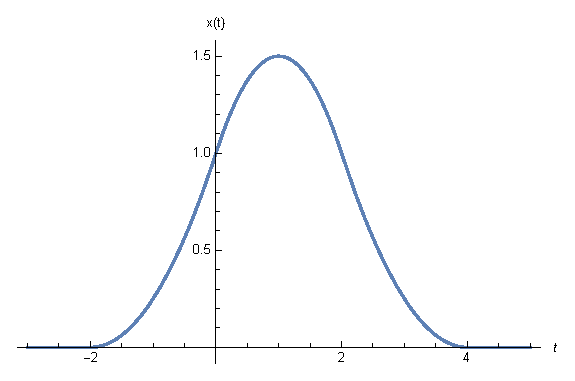
\includegraphics[width=0.8\textwidth]{12-9.eps}
    \end{center}
    \caption{Sketch of $x(t)=\mathrm{tri}(\frac{\tau}{2})*\mathrm{rect}(\frac{\tau-1}{2})$.}
\end{figure}

13.

(a) The impulse response is
$$h(t)=\int_{-\infty}^t(t-\tau)e^{-(t-\tau)}\delta(\tau)\mathrm{d}\tau=\int_{-\infty}^tte^{-t}\delta(\tau)\mathrm{d}\tau=te^{-t}u(t).$$
An LTI system is causal iff its impulse response $h(t)=0$ for all $t<0$. Since $h(t)=0$ for all $t<0$, the system is $\boxed{\text{causal}}$.

An LTI system is BIBO stable iff its impulse response is absolutely integrable.
$$\int_{-\infty}^\infty|h(t)|\mathrm{d}t=\int_0^\infty te^{-t}\mathrm{d}t=-(t+1)e^{-t}\bigg|_0^\infty=1.$$
i.e. its impulse response is absolutely integrable, $\int_{-\infty}^\infty|h(t)|\mathrm{d}t<\infty$. Therefore, the system is $\boxed{\text{stable}}$.

An LTI system is memoryless or stable iff its impulse response is $h(t)=a\delta(t)$. Since $h(t)$ cannot be $a\delta(t)$ for any $a$, the system is $\boxed{\text{NOT static}}$.% In fact, it is an IIR system because $h(t)$ persists infinitely.

(b) The impulse response is
$$h(t)=\int_{t-1}^{t+1}e^{-2(t-\tau)}\delta(\tau)\mathrm{d}\tau=\int_{t-1}^{t+1}e^{-2t}\delta(\tau)\mathrm{d}\tau=\mathrm{rect}\bigg(\frac{t}{2}\bigg)e^{-2t}.$$
Since $\exists t\ h(t)\neq0$ for $t<0$, the system is $\boxed{\text{NOT causal}}$.
$$\int_{-\infty}^\infty|h(t)|\mathrm{d}t=\int_{-1}^1e^{-2t}\mathrm{d}t=-\frac{1}{2}e^{-2t}\bigg|_{-1}^1=e^2-e^{-2}<\infty.$$
Since its impulse response is absolutely integrable, the system is $\boxed{\text{stable}}$.

Since $h(t)$ cannot be $a\delta(t)$ for any $a$, the system is $\boxed{\text{NOT static}}$.

14. We would first differentiate $x(t)$:
\begin{align*}
    \frac{\mathrm{d}}{\mathrm{d}t}x(t)&=\frac{\mathrm{d}}{\mathrm{d}t}[2e^{-3t}u(t-1)]\\
    &=2e^{-3t}\delta(t-1)+2u(t-1)(-3)e^{-3t}\\
    &=2e^{-3t}\delta(t-1)-6e^{-3t}u(t-1)\\
    &=2e^{-3}\delta(t-1)-3x(t)
\end{align*}
Then, $\frac{\mathrm{d}x(t)}{\mathrm{d}t}=2e^{-3}\delta(t-1)-3x(t)\rightarrow2e^{-3}h(t-1)-3y(t)$. Besides, $\frac{\mathrm{d}x(t)}{\mathrm{d}t}\rightarrow e^{-2t}u(t)-3y(t)$, we have
$$2e^{-3}h(t-1)=e^{-2t}u(t)$$
Let $s=t-1$, then
$$h(s)=\frac{e^3}{2}e^{-2(s+1)}u(s+1)=\frac{1}{2}e^{-2s+1}u(s+1)$$
Therefore, the impulse response $h(t)$ of $S$ is
$$\boxed{h(t)=\frac{1}{2}e^{-2t+1}u(t+1)}$$

15.

(a) We have enough information to determine the output $y(t)$.
$$\boxed{y(t)=x(t)*h(t)=2x_0(t)*h_0(t)=2(x_0(t)*h_0(t))=2y_0(t)}$$
\begin{figure}[H]
    \begin{center}
        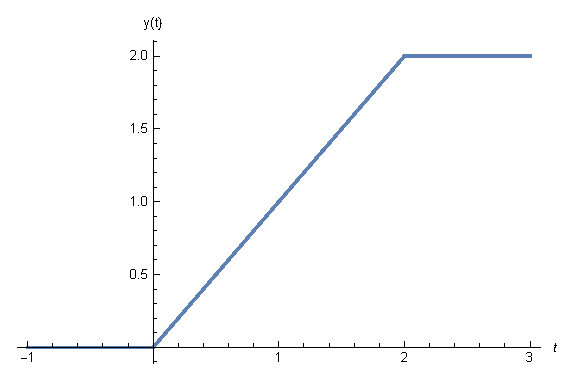
\includegraphics[width=0.6\textwidth]{15(a).eps}
    \end{center}
    \caption{15(a).}
\end{figure}

(b) We have enough information to determine the output $y(t)$.
\begin{align*}
    y(t)&=x(t)*h(t)\\
    &=(x_0(t)-x_0(t-2))*h_0(t+1)\\
    &=(x_0(t)*h_0(t+1))-(x_0(t-2)*h_0(t+1))\\
    &=\boxed{y_0(t+1)-y_0(t-1)}
\end{align*}
\begin{figure}[H]
    \begin{center}
        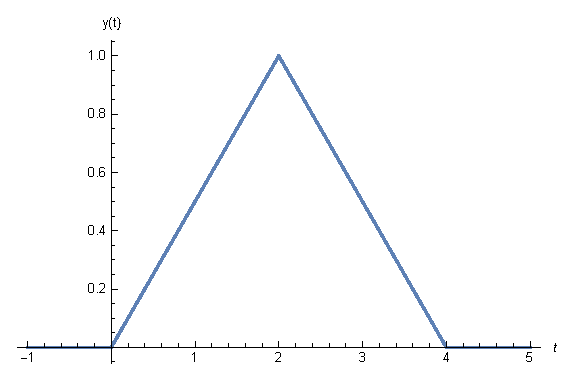
\includegraphics[width=0.6\textwidth]{15(b).eps}
    \end{center}
    \caption{15(b).}
\end{figure}

%(c) We have enough information to determine the output $y(t)$.
%$$\boxed{y(t)=x(t)*h(t)=x_0(t-2)*h_0(t+1)=y_0(t-2+1)=y_0(t-1)}$$
%\begin{figure}[H]
%    \begin{center}
%        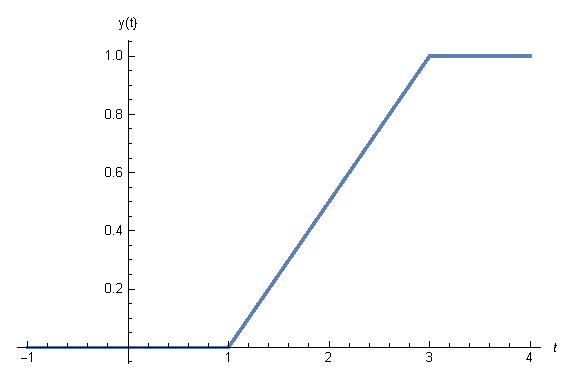
\includegraphics[width=0.6\textwidth]{15(c).eps}
%    \end{center}
%    \caption{15(c).}
%\end{figure}

(c) Try express $y(t)$ in terms of $x_0(t)$ and $h_0(t)$
$$y(t)=x(t)*h(t)=x_0(-t)*h_0(t)$$
Since the convolution does not exist, we do not have enough information to determine the output $y(t)$.

(d) We have enough information to determine the output $y(t)$.
$$\boxed{y(t)=x(t)*h(t)=x_0(-t)*h_0(-t)=y_0(-t)}$$
\begin{figure}[H]
    \begin{center}
        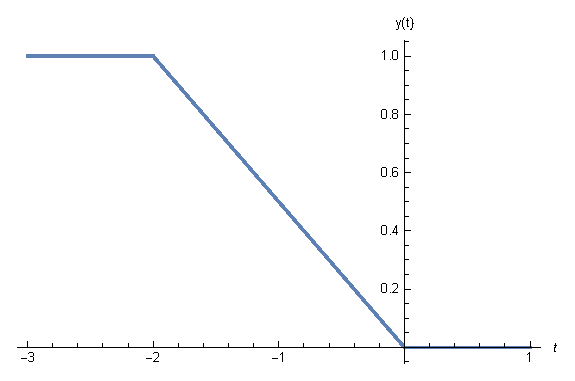
\includegraphics[width=0.6\textwidth]{15(e).eps}
    \end{center}
    \caption{15(e).}
\end{figure}

(e) We have enough information to determine the output $y(t)$.
$$\boxed{y(t)=x(t)*h(t)=x_0'(t)*h_0(-t)=y_0'(t)}$$

(f) We have enough information to determine the output $y(t)$. Using the result from Problem 7(b),
$$y(t)=x(t)*h(t)=x_0'(t)*h_0'(t)=y_0''(t)$$
%To find out the convolution we only need to consider the nonzero range of $y_0(t)$ that is
We first find the expression of $y_0(t)$
$$y_0(t)=\frac{1}{2}(tu(t)-(t-2)u(t-2))$$
Then we can calculate its derivatives of $y_0(t)$
$$y_0'(t)=\frac{1}{2}(u(t)-u(t-2))$$
$$y_0''(t)=\frac{1}{2}(\delta(t)-\delta(t-2))$$
Hence,
$$\boxed{y(t)=\frac{1}{2}(\delta(t)-\delta(t-2))}$$
\begin{figure}[H]
    \begin{center}
        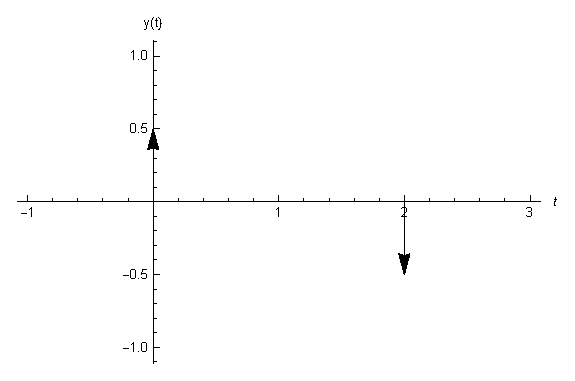
\includegraphics[width=0.6\textwidth]{15(f).eps}
    \end{center}
    \caption{15(f).}
\end{figure}

16. Find natural response $y_h(t)=Ce^(st)$.
$$\frac{\mathrm{d}t}{\mathrm{d}t}y_h(t)+10y_h(t)=0$$
$$\Longrightarrow10Ce^{st}+sCe^{st}=0$$
$$\Longrightarrow s=-10$$
$$\Longrightarrow y_h(t)=Ce^{-10t}$$
We analyze a unit-step input signal
\[x(t)=u(t)=
    \begin{cases}
        1,&t\geq0\\
        0,&\text{otherwise}
    \end{cases}
\]
Since $x(t)=0$ for $t\leq0$, the condition of initial rest implies the auxiliary condition $y(t)=0$ for $t\leq0$.

Since $x(t)=1$, $\frac{\mathrm{d}}{\mathrm{d}t}x(t)=0$ for $t\geq0$, the forced response is
$$y_p(t)=P\ \text{for}\ t\geq0$$
Thus
$$y(t)=y_h(t)+y_p(t)=Ce^{-10t}+P\ \text{for}\ t\geq0$$
Plugging into the diffeq yields:
$$10Ce^{-10t}+10P-10Ce^{-10}t=2\ \text{for}\ t\geq0$$
$$\Longrightarrow P=\frac{1}{5}$$
Furthermore, using the initial condition $y(0)=1$,
$$Ce^0+P=1$$
$$\Longrightarrow C+\frac{1}{5}=1$$
$$\Longrightarrow C=\frac{4}{5}$$
Therefore, the expression of response of the CT system is
\[\boxed{y(t)=
    \begin{cases}
        \frac{4}{5}e^{-10t}+\frac{1}{5},&t\geq0\\
        0,&t<0
    \end{cases}
    =\bigg(\frac{4}{5}e^{-10t}+\frac{1}{5}\bigg)u(t)}
\]
\end{document}